%%%%%%%%%%%%%%%%%%%%%%%%%%%%%%%%%%%%%%%%%%%%%%%%%
% Relatório Final - Projeto de Pesquisa
% Métodos de Otimização
% Baltz & Machado
% Capítulo 2
%%%%%%%%%%%%%%%%%%%%%%%%%%%%%%%%%%%%%%%%%%%%%%%%%


\chapter{\Large{Métodos Clássicos de Otimização}}\label{chp:2}


\section{{O Método de Newton}}

\hspace{0.8cm}

\subsection{Entendendo o Método}

%TODO: Falar de funções bem definidas

O Método de Newton, foi desenvolvido com o objetivo de realizar a estimativa
para as raízes de uma função. De modo que, a execução do método é feita de
forma iterativa, repetindo sempre o mesmo processo, atualizando o mesmo valor.

Este método faz uso do recurso de derivação, existindo, uma relação muito
forte com o ângulo da reta tangênte ao ponto, na função. Ademais, é
importante ressaltar, que é necessário um palpite inicial, que represente
o valor de \textit{x}, no qual, partindo desse valor, será buscado a raiz da
função. E com isso, vamos entender como o dado método funciona:

Partindo do princípio do método, o objetivo será utilizar a reta tangente a um
ponto, para gerar valores cada vez mais próximos da raiz daquela função. De
modo que, será analisado a inteseção da reta tangente com o eixo das
abscissas. E sendo a diferenca do valor x da entrada da função com o valor de
interseção no eixo x, o novo valor de entrada na função, constuindo assim
várias iterações, gerando valores cada vez mais próximos da raiz. Como será
visto, a seguir:

Já sabido que a equação da reta é dada como:

\begin{equation}
    (y-y_0)=m(x-x_0).
\end{equation}

E levando em conta que temos como objetivo encontrar $x$, que é um ponto
sobreposto no eixo x, podemos considerar $y=0$, logo:

\begin{equation}
    -y_0=m(x-x_0).
\end{equation}

Com isso, sabemos que $y_0$ é a imgam da função $f(x_0)$, e $m$ é o ângulo da
reta tangênte ao ponto $x_0$, ou seja: $m=f'(x_0)$. Logo, desenvolvendo essa
equação, temos:

\begin{equation}
    -f(x_0) = f'(x_0)(x-x_0),
\end{equation}

\begin{equation}
    -f(x_0) = f'(x_0)x - f'(x_0)x_0,
\end{equation}

\begin{equation}
    0 = f'(x_0)x - f'(x_0)x_0+f(x_0),
\end{equation}

\begin{equation}
    0 = x - x_0 + \frac{f(x_0)}{f'(x_0)},
\end{equation}

\begin{equation}
    x = x_0 - \frac {f(x_0)}{f'(x_0)}.
\end{equation}\\

E com isso, exemplificando em um gráfico, temos:

Sendo $f(x)=-x^2+2x$, o palpite inicial $x_0=1.5$, $P1$ sendo o ponto de que
representa $x_0$ aplicado a função $f$ e $x1$ a interseção da reta tangente à
$P1$ com o eixo x.

\begin{figure}[ht]
    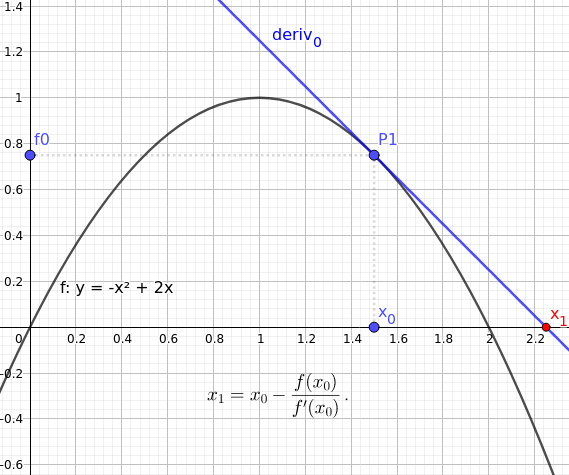
\includegraphics[width=0.55\textwidth]
      {src/MetodoNewton_grafico_1.png}
    \centering
    \caption{
      \centering
      Primeira iteração do Método de Newton.
    }
    \label{MetodoNewton_grafico_1}
\end{figure}


E a partir do dado gráfico, agora podemos entender melhor como a iteração
funcionará, pois, e valor gerado, $x_1$, será aplicado no mesmo método. E com
isso, podemos construir a seguinte equação:

\begin{equation}
    x_{k+1} = x_{k} - \frac {f(x_{k})}{f'(x_{k})}.
    \label{newton_primeiraDeriv}
\end{equation}

E com isso, gera-se uma sequência $\{xk\}$, donde, esta, converge para a raiz
da função. E nesse sentido, vejamos a próxima iteração (Figura
\ref{MetodoNewton_grafico_2}) do exemplo mostrado na Figura
\ref{MetodoNewton_grafico_1}.

\begin{figure}[ht]
    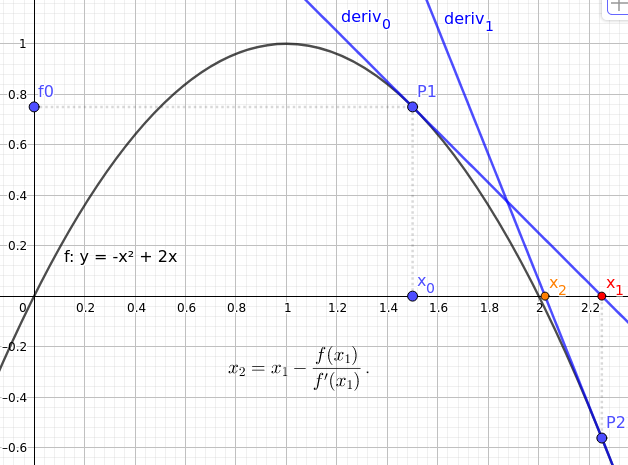
\includegraphics[width=0.55\textwidth]
      {src/MetodoNewton_grafico_2.png}
    \centering
    \caption{
      \centering
      Segunda iteração do Método de Newton.
    }
    \label{MetodoNewton_grafico_2}
\end{figure}

E assim, podemos notar a aproximação de $x_k$ para a raiz de $f$, observando o
ponto $x_2$.

Ademais, é válido ressaltar que o denominador da equação
\ref{newton_primeiraDeriv} tem que ser diferente de 0 (ou seja, a reta tengante
num ponto $P$ não pode ser paralela ao eixo x). No entanto, caso contrário,
isso significa que a dada função não possui raiz na proximidade daquele ponto.

\subsection{Encontrando Mínimos}

E é dessa maneira que, agora, podemos utilizar este método para encontrar
mínimos de uma função. Vimos que, o Método de Newton calcula raízes, e
desse modo, vinculando o que foi estudado no Capítulo 1, sabemos que, os
mínimos de uma função podem ser representados como raízes de sua derivada.

%TODO: Falar mais/melhor sobre a sequencia {xk} (tendencia ao 0 da funcao)

Então, dado que as raizes de $f(x)$ podem ser geradas a partir da equação
\ref{newton_primeiraDeriv}, temos que, considerando $g(x)$ uma função duas vezes
derivável, e tendo como objetvido encontrar seus pontos de mínimo, pode-se
utilizar o Método de Newton para resolver tal problema da seguinte forma:

\begin{equation}
    x_{k+1} = x_{k} - \frac {g'(x_{k})}{g''(x_{k})}.
\end{equation}

Encontrando então as raizes aproximadas de sua derivada, e considerando
estas como  $x^*$, temos então que:

\begin{equation}
    g(x^*) = 0.
\end{equation}

O método é simples, entrega muitas vezes ótimos locais próximos ao ponto
inicial, mas tem seu destaque pode ser curto e facilmente computável.

Problemas de maximização podem ser vistos sob o seguinte olhar:

\begin{equation}
    max(f(x)) = min(-1 * f(x))
\end{equation}

Que com isto podem ser otimizados pelo Método de Newton também.

O movimento de \(x_k\) dentro da sequência, é determinado pela relação das
quantidades e propriedades que tanto a primeira quanto a segunda derivada
oferecem. As quantidades determinam a velocidade do motivento, e os sinais
indicam a direção do movimento. De certa forma podemos ver esse movimento da
sequência \(\{x_k\}\) como instantes do movimento de uma bola numa ladeira, que
no começo de sua descida é acelerada, e, conforme chega ao plano no fim da
ladeira, começa a reduzir sua velocidade, até supostamente chegar no ponto mais
baixo.


\section{{Outros Métodos}}

\hspace{0.8cm}

\section{{Programando os Métodos}}

\hspace{0.8cm}

\textbf{Método de Newton}

A forma mais simples e mais util de implementar o metodo de Newton é na forma
de busca das raízes, que uma vez  implementada, só precisamos por como entrada
a priemira e a segunda derivada da função que desejamos minimizar, já que o
método não precisa saber qual a função de fato. A seguir temos a implementação
na liguagem de programação Rust:

\begin{lstlisting}
pub fn newton1x1<F>(funcao_derivada: &F, x: f64) -> (usize, f64)
where
    F: Fn(f64) -> f64,
{
    let mut entrada_atual = x;
    let maximo_iteracoes = 100;

    for iteracao_atual in 1..=maximo_iteracoes {
        let diferenca: f64 =
            funcao_derivada(entrada_atual.clone())
            /
            derive1x1(&funcao_derivada, &entrada_atual);

        println!("diferenca: {}", diferenca);
        entrada_atual -= diferenca;

        if diferenca.abs() < 0.0000001 {
            return (iteracao_atual, entrada_atual);
        }
    }

    return (maximo_iteracoes, entrada_atual);
}
\end{lstlisting}


Os parâmetros da função são:

    \begin{itemize}
            \item Uma função \(f : \mathbb{R} \rightarrow \mathbb{R}\)
            \item Uma entrada x sendo o chute inicial do otimo.
    \end{itemize}


A função derive1x1 recebe como parametro uma função e um ponto, tendo como
retorno a derivada da função entregue, no ponto especificado. Restingindo-se
à funções do tipo \(f : \mathbb{R} \rightarrow \mathbb{R}\), donde deve ser
escrita pelo úsuario como bem entender.



\textcolor[rgb]{1,0,0}{\section{{O Método de Newton para Várias Variáveis}}}
